\section{Method}
\label{sec:method}

\begin{figure*}[t]
\centering
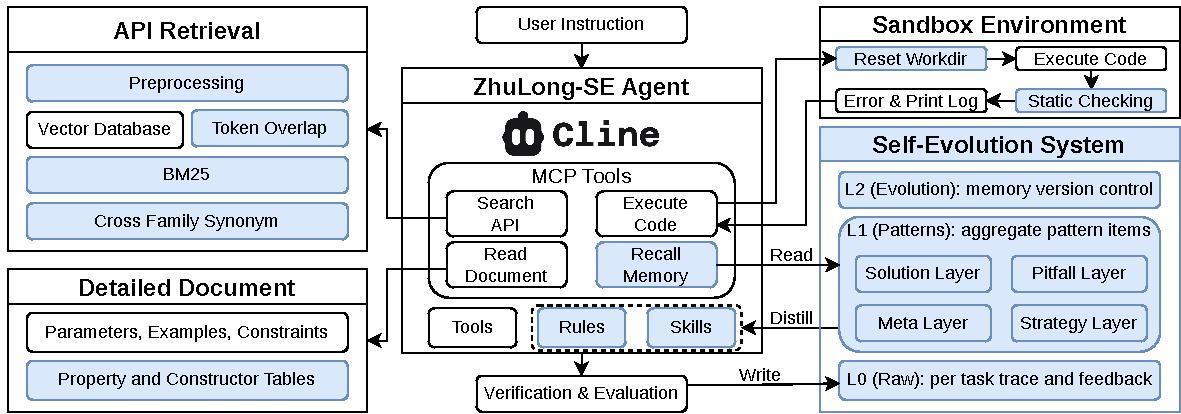
\includegraphics[width=1.0\textwidth]{figures/zhulong-se.pdf}
\caption{Architecture of ZhuLong-SE, adapted from the ZhuLong execution framework~\cite{liu2026zhulong}. Blue-highlighted blocks denote components added or enhanced in this work. Unhighlighted blocks show the shared execution workflow.}
\label{fig:architecture}
\end{figure*}

Building on the origin ZhuLong execution harness~\cite{liu2026zhulong}, ZhuLong-SE retains its retrieval--documentation--execution loop and introduces the blue-highlighted extensions in Figure~\ref{fig:architecture}: enhanced API retrieval and documentation, isolated parallel sandbox management, a precision-optimized static checker, human-crafted rules and skills, and an offline cross-task self-evolution system. We describe the task-level harness extensions in Sections~\ref{sec:method_retrieval}--\ref{sec:method_experience}, followed by self-evolution in Section~\ref{sec:selfev}.
% ZhuLong-SE建立在ZhuLong执行框架~\cite{liu2026zhulong}之上，保留其“检索—文档—执行”闭环，并引入图~\ref{fig:architecture}中以蓝色标出的扩展：增强的API检索与文档、隔离并行沙箱管理、精度优化静态检查器、人工编写的规则与技能，以及离线跨任务自进化系统。我们首先在第~\ref{sec:method_retrieval}至~\ref{sec:method_experience}节介绍任务级框架扩展，随后在第~\ref{sec:selfev}节介绍自进化系统。

\subsection{API Retrieval}
\label{sec:method_retrieval}

ZhuLong provides a single \texttt{search\_apis} MCP tool that uses semantic retrieval~\cite{liu2026zhulong}. ZhuLong-SE retains its embedding-based semantic path, adds a dedicated keyword-oriented tool (\texttt{search\_apis\_by\_keyword}), and supplements matches missed by the summary with a BM25 pass over the full description text. The keyword path targets queries that the semantic index handles poorly, such as abbreviations and camel-case fragments. The index tokenizes each API name by splitting on camel-case boundaries and stripping family prefixes. The query is bidirectionally expanded for abbreviations (e.g., CV$\leftrightarrow$CellView, crt$\leftrightarrow$create), enabling matches on abbreviated tokens inside API names. Depending on query type, a router expands abbreviations, returns direct-match hints for API-name fragments, or appends semantic results for natural-language queries. Finally, a cross-family synonym map links four functionally equivalent API families (db*, emy*, goa*, ae*), so a hit in one family surfaces equivalents in the others, addressing the failure mode where an agent recalls the correct operation but selects the wrong interface family.
% ZhuLong通过单一的\texttt{search\_apis}工具使用语义检索~\cite{liu2026zhulong}。ZhuLong-SE保留其基于嵌入的语义路径，新增专用的关键词工具\texttt{search\_apis\_by\_keyword}，并通过对完整描述文本的BM25检索补充摘要遗漏的匹配。关键词路径针对语义索引处理不佳的查询，如缩写和驼峰片段。索引通过驼峰边界拆分API名称并去除族前缀；查询则双向扩展缩写（例如CV$\leftrightarrow$CellView，crt$\leftrightarrow$create），从而匹配API名称中的缩写词元。路由器根据查询类型扩展缩写、为API名称片段返回直接匹配提示，或为自然语言查询追加语义检索结果。最后，一个跨族同义词映射连接四个功能等价的API族（db*、emy*、goa*、ae*），使命中一族时同时呈现其他族的等价项，解决智能体记得正确操作但选错接口族的问题。

\subsection{Documentation Enrichment}
\label{sec:method_doc}

ZhuLong's \texttt{get\_api\_details} returns parameter types, return values, examples, and inferred constraints~\cite{liu2026zhulong}, but its per-API pages do not expose class instance properties. ZhuLong-SE therefore parses the raw documentation into a property table and appends it to each detailed response, so a queried class exposes its instance attributes alongside its methods. Constructor notes also disambiguate ambiguous calls: for example, \texttt{emyPointArray} accepts a plain list of points, a fact the per-signature page does not state.
% ZhuLong的\texttt{get\_api\_details}返回参数类型、返回值、示例和推断出的约束~\cite{liu2026zhulong}，但其逐API页面不公开类的实例属性。ZhuLong-SE因此将原始文档解析为属性表并附加到每个详细响应，使查询到的类在方法之外也暴露实例属性。构造函数注释还消除了模糊调用的歧义：例如，\texttt{emyPointArray}接受普通点列表，而逐签名页面并未说明这一事实。

\subsection{Sandbox Execution}
\label{sec:method_sandbox}

We run multiple isolated sandbox endpoints, each with an independent working directory, and dispatch requests through a queue pool. A routine clears working directories before each run and resets library files to minimal content, so prior runs do not bias subsequent ones. This isolation ensures that execution feedback reflects the current code under test, not residual state from earlier tasks. The queue pool enables concurrent evaluation without changing ZhuLong's per-task interaction protocol~\cite{liu2026zhulong}.
% 我们运行多个隔离的沙箱端点，每个端点拥有独立工作目录，并通过队列池分派请求。一个例行程序在每次运行前清空工作目录并将库文件重置为最小内容，使先前运行不会影响后续运行。这种隔离确保执行反馈反映当前被测试代码，而非先前任务的残留状态。队列池在不改变ZhuLong逐任务交互协议~\cite{liu2026zhulong}的前提下支持并发评估。

\subsection{Static Checking}
\label{sec:method_checker}

Because PyAether's SWIG bindings expose all symbols at import time regardless of whether the underlying function exists at runtime, an agent may call a fabricated API or pass a native Python value where a SWIG-wrapped type is required without triggering any runtime error during self-test—yet the submission fails the hidden test that exercises that path. To catch such failures before submission, we introduce a static checker that runs after the agent's self-test and before final submission.
% 由于PyAether的SWIG绑定在导入时暴露所有符号，而不管底层函数在运行时是否存在，智能体可能调用捏造的API或将原生Python值传递给需要SWIG封装类型的位置，而不会在自测期间触发任何运行时错误——但提交会在执行该路径的隐藏测试中失败。为了在提交前捕获此类失败，我们引入了一个静态检查器，在智能体自测之后、最终提交之前运行。

The checker parses submitted code into an abstract syntax tree, extracts API calls, and checks four documented misuse patterns: (i) fabricated APIs, (ii) incorrect keyword arguments, (iii) native Python values passed where explicit SWIG-wrapped construction is required, and (iv) silently swallowed exceptions. Actionable findings are returned to the agent for repair before final submission. The rules are derived from the API documentation and refined on real submissions. As a reference-code sanity check, the checker raises no flags on any of the 158 ground-truth solutions. This result is limited to that set and is not a general zero-false-positive guarantee.
% 检查器将提交的代码解析为抽象语法树，提取API调用，并检查四类已记录的误用模式：（i）捏造的API，（ii）错误的关键字参数，（iii）传递给需要显式SWIG封装构造的参数的原生Python值，以及（iv）被吞没的异常。可操作的发现被返回给智能体，以便在最终提交前修复。规则来源于API文档，并在真实提交上进行精炼。作为参考代码的健全性检查，检查器未对158个ground-truth解中任何一个标记问题；此结果仅限于该集合，并非一般性的零误报保证。


\subsection{Human-Crafted Experience}
\label{sec:method_experience}

ZhuLong-SE additionally injects four skills and one rule file authored from PyAether development experience rather than specific benchmark solutions. The skills cover API search, command-family selection, interpretation of silent or ambiguous sandbox feedback, and explicit SWIG type construction. The rule file requires API-detail checks before use, post-creation verification, and bounded search, providing a stable prior that complements knowledge learned from the execution traces.
% ZhuLong-SE还注入四条技能和一条规则文件，这些内容来源于PyAether开发经验而非基准任务的解答。技能涵盖API搜索、命令族选择、静默或模糊沙箱反馈的解读，以及显式SWIG类型构造。规则文件要求在使用前进行API详情检查、创建后验证和有限搜索，提供了一个稳定的先验知识，与执行轨迹学到的知识形成互补。
